\documentclass{article}   	                         % use "amsart" instead of "article" for AMSLaTeX format
\usepackage{fullpage}                		% ... or a4paper or a5paper or ... 
\usepackage{enumerate}				% Use enumerate to list subsections
\usepackage{graphicx}				% Use pdf, png, jpg, or eps§ with pdflatex; use eps in DVI mode
\usepackage{caption}
\usepackage{fancyvrb}
\usepackage{amsmath}
\usepackage{dsfont}
\newcommand{\ra}{\rightarrow}

%SetFonts

\title{Computer System Fundamentals HW \#5}
\author{Quan Zhou}
\date{Mar 19th, 2016}
\begin{document}
\maketitle
\section*{Problem 1}
\begin{BVerbatim}
F-SCAN CPU scheduler where the CPU uses SJF algorithm on high-priority buffer
\end{BVerbatim}
\\
\\
We could regard this scheduler as a two-queue M/G/1 system where the serving time follows a uniform distribution and each queue has an unlimited buffer size. The service time follows a uniform distribution with low bound of 1ms and higher bound of 20 ms. Then we can derive:\\
\begin{equation} \mathds{E}(T_s) = \frac{1}{2}\left(T_s(low) + T_s(High)\right) = \frac{1}{2}(0+19) = 9.5 \text {  msec}\end{equation} 
\begin{equation} \text{Var}(T_s) = \frac{1}{12}\left(T_s(High) - T_s(Low)\right) = \frac{1}{12}(19^2) = \frac{361}{12} \text {  msec}\end{equation} 
\begin{equation} \sigma_{T_s} = \sqrt(\text{Var}(T_s)) =  5.485 \text {  msec}\end{equation} 
\begin{equation}\rho = \lambda T_s = (0.1 \text {  requests per ms} )(9.5 \text {  ms} ?= 0.95 \end{equation}
So at steady state, a request R arriving in the system and in the worst case it just misses the high-priority queue and therefore will be waiting in the low-priority queue. In this scenario, the expected value of requests to be served before R gets served is equal to the total requests in the system, or $q$. Therefore, we have the following equation:\\
\begin{equation} A = \frac{1}{2}\left[1 + \left(\frac{\sigma_{T_s}}{T_s}\right)^2\right] = \frac{1}{2}(1 + 0.333) = 0.667\end{equation}
\begin{equation} q = \frac{\rho^2 A}{1 - \rho} + \rho = \frac{(0.95^2)(0.667)}{1- 0.95} + 0.95 = 13.0 \text{  requests} \end{equation}  
So $T_q = \frac{13}{100} = 0.13$\\
Therefore, the expected value of the maximum number of out-of-order executions of jobs in this system is:\\
\begin{equation}\frac{1}{2}(100)(T_q) = 6.5 \text{    requests}\end{equation}
\section*{Problem 2}
\begin{BVerbatim}
Codes please see src/problem2/Controller.java
\end{BVerbatim}
\\
\begin{BVerbatim}
To test each type of scheduler, go to MM1System and change the interger schedulertype to 1-4
\end{BVerbatim}
From the codes we generate the following diagrams:\\
\begin{figure}
\centering
\begin{minipage}{.5\textwidth}
  \centering
  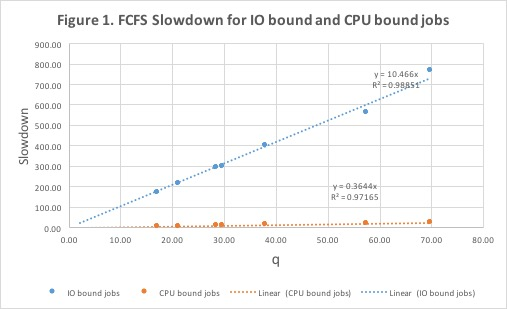
\includegraphics[width=\linewidth]{Picture1.jpg}
  \captionof{figure}{FIFO/FCFS scheduler}
  \label{fig:FIFO/FCFS}
\end{minipage}%
\begin{minipage}{.5\textwidth}
  \centering
  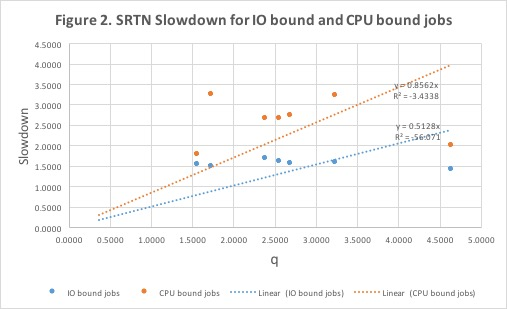
\includegraphics[width=\linewidth]{Picture2.jpg}
  \captionof{figure}{SRTN scheduler}
  \label{fig:SRTN}
\end{minipage}
\end{figure}

\begin{figure}
\centering
\begin{minipage}{.5\textwidth}
  \centering
  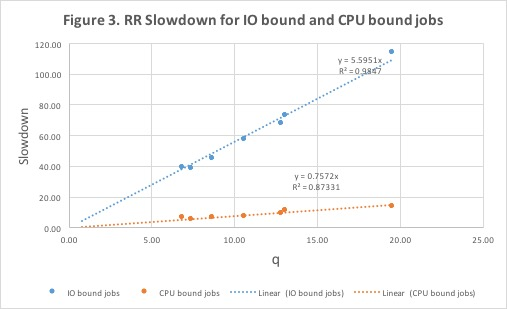
\includegraphics[width=\linewidth]{Picture3.jpg}
  \captionof{figure}{RR scheduler}
  \label{fig:RR}
\end{minipage}%
\begin{minipage}{.5\textwidth}
  \centering
  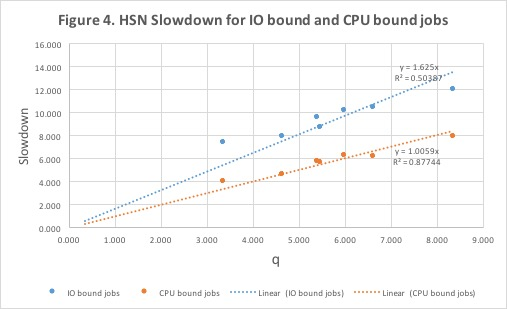
\includegraphics[width=\linewidth]{Picture4.jpg}
  \captionof{figure}{HSN scheduler}
  \label{fig:HSN}
\end{minipage}
\end{figure}

The numbers are generated by running the code with a summary of results at the end of simulations. I copy paste the numbers into excel and for each scheduler I plotted the slowdown versus the average (or steady state) number of requests in the system. From the perspective of  I/O bound jobs, they would prefer Shortest Remaining Time Next (SRTN), then Highest Slowdown Next (HSN), then Round Robin (RR) and lastly First Come First Serve (or FIFO). The reason is because the I/O bound jobs are usually arrives frequently and takes less time compared to CPU bound jobs. SRTN makes the best option for I/O bound jobs.
\section*{Problem 3}
\begin{enumerate}[(a)]
\item
In this scheduler design, it seems the server prefers the files that with larger IDs.\\
For example, assuming the cache has three files with IDs 4,5,6, $Q_1$ is empty whereas in $Q_2$ there are files queued up with the IDs in the following order:  5, 7, 2, 1, 8. Then the server would fetch file ID = 7 and store in the cache; meanwhile, it replaces the file ID = 4 (as the smallest ID). If we continue this operations, we can find the cache would never pick/select files with small IDs (especially those that are smaller than that of the files in the cache) in the queue. Therefore, it is not a fair design for HTTP requests scheduler.
\item
N-step/batched scan
\item
Performance wise, larger N would be better: the scheduler would be more efficient in picking those files with larger IDs, but would do so at the cost of longer time to be served (head stickiness).
\item
Fairness wise, smaller N would be better: with a finite amount of number of requests in the higher priority buffer, all requests, whether files with large ID or smaller ID are guaranteed to be served.
\item
\begin{enumerate}[1.]
\item The load on the system is light and a small number of files are highly popular compared to the rest\\
N = 100,  
\item The load on the system is moderate and a small number of files are highly popular compared to the rest\\
N = 100, like the case above, only few non-cached file requests will come. Since it is just a medium load, it is unlikely for a non-cached file to be served last resulting in lots of requests being queued up.
\item The load on the system is high and all files in the system are equally likely to be requested\\
N = 1, since all files are equally likely to be requested, we need a fairer scheduling to guarantee all requests are being served. Since the files requested will most likely not be in the cache, there is no need to serve smaller files first.
\item The load on the system is extremely high and a small number of files are highly popular compared to the rest\\
In this case of extremely heavy loaded system, it is likely for a non-cached file to be served last resulting in lots of requests being queued up using a large N-batch scheduling. Also, low N would would be bad as it is highly likely the files requested will not be in the cache. To balance performance and fairness, it would make sense to choose N =10.
\end{enumerate}
\end{enumerate}
\section*{Problem 4}
\begin{BVerbatim}
3 classes of jobs in a computer system
\end{BVerbatim}
\begin{enumerate}[(a)]
\item
Starvation is possible, and class C is mostly susceptible to the preemptive scheduling: Since class B could arrive to the system frequently, the queue maybe mostly Bs and a little bit of As and all Cs have to wait for As and Bs to finish. It would take really long time before the lowest priority job (class C) get served. 
\item
$\lambda_A = \frac{1}{60} \text {  request/sec}$, $T_s (A) = 5 \text {  sec}$\\
$\lambda_B = 1 \text {  request/sec}$, $T_s (B) = 0.5 \text {  sec} $\\
$\lambda_C = \frac{1}{300} \text{  request/sec}$, $T_s (C) = 20 \text {  sec}$\\
\begin{BVerbatim}
For class A jobs:
\end{BVerbatim}
\\
because class A jobs have the highest priorities and therefore they are served in the fashion of FCFS. So worst case response time for A is: \\
$\textbf {5 seconds}$\\
\begin{BVerbatim}
For class B jobs:
\end{BVerbatim}
\\The worst case is when there is a class A scheduled before the arrival of a class B job. So $T_w(B) = 5 \text {  sec}$. so we get the worst case response time for A :\\
$\textbf {5.5 seconds}$\\
\begin{BVerbatim}
For class C jobs:
\end{BVerbatim}
\\
First of all, it arrives the same time as class A job arrives. So C has to wait for A, which will take 5 seconds.Then during the waiting, class B jobs could arrive (say one each second, so there would be 5 class B jobs arriving during the 5 second waiting). They will be scheduled before the class C job can proceed. So C has to wait another $5\times (0.5 \text {  seconds}$ or 2.5 seconds. Lastly during the execution, we need 20 sec of interleaved execution with arriving jobs B. So it will take actually 40 sec. so we get the worst case response time for C:\\
$\textbf {5+2.5+40 = 47.5 seconds}$\\
\item
based on how this scheduler prioritize different classes of jobs, we obtained the following utilization equation:\\
\begin{equation}5\left(\frac{1}{60}\right) + 0.5(1) +c\left(\frac{1}{300}\right) \leq 1 \end{equation}
solve for c and we get 125 seconds, which is the maximum amount of CPU time per period for jobs of class C that the system could reach steady state. Beyond that, steady state won't be possible.\\
\item
Suppose job class C is running and using resource R. If a job class A arrives during that time and needs to use R, it cannot use R since C holds R even though C is preempted on the CPU. Thus, A will have to wait, which compromises the priority rules.
\item
Suppose class A, B and C arrives continuously, with class C job start running right before A arrives in the system. For C and B to finish the interleaved execution, it takes 40 seconds. So worst case response time for A is 45 seconds.\\
\item
Priority inversion means that a higher priority process is forced to wait for a lower priority process. For example, in the above problem with resource R, A waits for lower priority job C.\\
\item
In priority inheritance, a low priority process holding a shared resource will get the highest priority of all processes waiting for the resource. This ensures that the low-priority process will free up the shared resource as soon as possible.\\
\item
25 seconds. C inherits the highest priority and cannot be interrupted. A will wait for 20 seconds, which is the time a class C job needs to be executed; then A will execute for 5 seconds; add the two together we get 25 seconds.
\end{enumerate}
\end{document}